\begin{figure}

\begin{subfigure}{\linewidth}
\centering
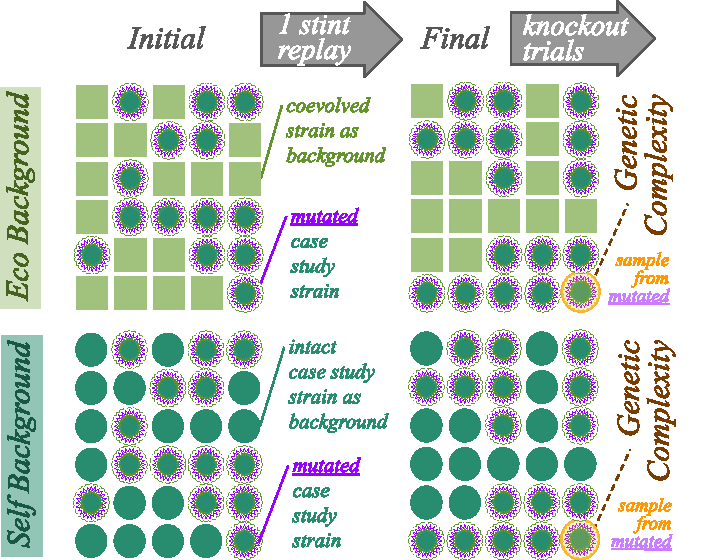
\includegraphics[width=0.85\linewidth]{img/mutagenized-replay-schematic.pdf}
~~

\caption{%
\footnotesize
replay trial design
}
\label{fig:replay-background:design}
\end{subfigure}

% The phenotype panel's teeplot PDF is emitted on a landscape page with its
% content laid a quarter turn over (its PNG twin is upright), so it is turned
% back upright here.
% Note that `angle' is given before `height' so that the height applies to the
% graphic as rotated, not as stored.
\begin{subfigure}{0.22\linewidth}
\centering

\includegraphics[angle=90,height=1.22in]{../binder/binder-2026-09-01-replay-phenotypes.ipynb/binder/teeplots/2026-09-01-replay-phenotypes/hue=source+viz=pointplot+y=prop+ext=.pdf}
\end{subfigure}%
\begin{subfigure}{0.18\linewidth}
\centering

\includegraphics[height=1.22in,trim=0 0 4cm 0,clip]{../binder/binder-2025-11-26-replaysmutagenized50.ipynb/binder/teeplots/2025-11-26-replaysmutagenized50/clip=62+hue=bucket+inner=quart+viz=violinplot+x=bucket+y=is-less-fit+ext=.pdf}
\end{subfigure}%
\begin{subfigure}{0.30\linewidth}
\centering

\includegraphics[height=1.22in,trim=2cm 0 0 0,clip]{../binder/binder-2025-11-23-replaysmutagenized08.ipynb/binder/teeplots/2025-11-23-replaysmutagenized08/hue=bucket+inner=quart+viz=violinplot+x=bucket+y=is-less-fit+ext=.pdf}
\end{subfigure}%
\begin{subfigure}{0.30\linewidth}
\centering

\includegraphics[height=1.22in,trim=2.5cm 0 0 0,clip]{../binder/binder-2025-11-26-replaysmutagenized50.ipynb/binder/teeplots/2025-11-26-replaysmutagenized50/clip=62+hue=bucket+inner=quart+viz=violinplot+x=bucket+y=is-less-fit+ext=.pdf}
\end{subfigure}

\vspace{-0.75ex}
\begin{subfigure}{0.70\linewidth}
\footnotesize
\caption{8 mutation dose}
\label{fig:replay-background:moderatedose}
\end{subfigure}%
\begin{subfigure}{0.30\linewidth}
\footnotesize
\caption{50 mutation dose}
\label{fig:replay-background:highdose}
\end{subfigure}

\vspace{-2ex}
\caption{%
\textbf{Constructed niche selects to maintain genotype complexity.}
\footnotesize
We performed short one-round replay trials on the case study strain, in either co-evolved or self context.
To enhance standing variation and weaken inherent self-context effects, replay genomes were subject to moderate mutagenesis --- dosed to maintain some functionally intact genomes (\ref{fig:replay-background:design}).
Replays in self context maintained higher genotype complexity than co-evolved context (Mann-Whitney test, \ref{fig:replay-background:moderatedose}).
Self context likewise better preserved the case study strain's cigar-like morphology --- recovered from 51 of 69 replays, versus 29 of 69 under co-evolved context (risk ratio 1.76, Fisher's exact test; leftmost panel of \ref{fig:replay-background:moderatedose}).
By contrast, more intense mutagenesis did not reproduce this effect, suggesting specificity to preserve already-evolved complexity (Mann-Whitney test, \ref{fig:replay-background:highdose}\protect\footnotemark).
Supplementary Figure \ref{fig:replay-background-early} shows replay results for transfer rounds 0 to 34.
}
\label{fig:replay-background}

\end{figure}

% adapted from https://tex.stackexchange.com/a/67030
\footnotetext{%
For legibility, Figure \ref{fig:replay-background:highdose} clips an extreme outlier with 142-site genotype complexity observed from self-context replay (Supplementary Figure \ref{fig:replay-background-outlier}).
}
